% TU Delft beamer template
% Author: Erwin Walraven (initial version was created by Maarten Abbink)
% Delft Universiy of Technology

\documentclass{beamer}
\usepackage[english]{babel}
\usepackage{calc}
\usepackage[absolute,overlay]{textpos}
\usepackage{graphicx}
\usepackage{subfig}
\usepackage{amsmath}
\usepackage{amsfonts}
\usepackage{amsthm}
\usepackage{mathtools}
\usepackage{comment}
\usepackage{MnSymbol,wasysym}
\usepackage{url}
\usepackage{fancyhdr}
\usepackage{subfig}
\usepackage{xcolor}

%colors
\definecolor{mygray}{gray}{0.6}

\setbeamertemplate{navigation symbols}{} % remove navigation symbols
\mode<presentation>{\usetheme{tud}}

% BIB SETTINGS
\usepackage[backend=bibtex,firstinits=true,maxnames=30,maxcitenames=20,url=false,style=authoryear]{biblatex}
\bibliography{bibfile}
\setlength\bibitemsep{0.3cm} % space between entries in the reference list

% Commands
\renewcommand{\bibfont}{\normalfont\scriptsize}
\setbeamerfont{footnote}{size=\tiny}
\renewcommand{\cite}[1]{\footnote<.->[frame]{\fullcite{#1}}}
\newcommand{\sidenote}[1]{{\textcolor{mygray}{\emph{#1}}}}
\renewcommand{\exp}[1]{\langle #1 \rangle} %expectation

\title[]{Variational Quantum Eigensolver}
\institute[]{Technische Universiteit Delft, Nederland}
\author{Joost Bus \\ \tiny{j.c.p.bus@student.tudelft.nl}}
\date{\today}

\begin{document}
{
\setbeamertemplate{footline}{\usebeamertemplate*{minimal footline}}
\frame{\titlepage}
}
{\setbeamertemplate{footline}{\usebeamertemplate*{minimal footline}}}

% Overview
\begin{frame}{Overview}
\tableofcontents
\end{frame}

\section{General idea}
\begin{frame}{The general idea}
\begin{itemize}
	\item Operators that describe quantum systems grow exponentially with the system size. Finding the eigenvalues of such operators gets difficult very fast.
	\item Quantum Phase Estimation (QPE) can efficiently find the eigenvalue
	of a given eigenvector but requires fully coherent evolution.
	\item Variational Quantum Eigensolver (VQE) is an alternative algorithm that seeks to find (the lowest) eigenvalue of an operator, and its corresponding eigenstate using a hybrid algorithm which quantum parts are low depth and therefore requires less coherence.
\end{itemize}
\end{frame}

\section{Areas of application}
\begin{frame}{Areas of application}
	\begin{itemize}
		\item Chemistry \sidenote{original 2013 paper was about finding the ground state of He-H$^+$}
		\item Optimisation \sidenote{that's what we will be using it for}
	\end{itemize}
\end{frame}

\begin{frame}{Underlying mathematics}
	Any hamiltonian $\mathcal{H}$ can be written as
	\begin{equation}
		\mathcal{H} = \sum_{i, \alpha} h_\alpha^i\sigma_\alpha^i + \sum_{i, j, \alpha, \beta} h_{\alpha,\beta}^{i,j}\sigma_\alpha^i\sigma_\beta^j + \dots
	\end{equation}
	for real $h$ where Roman indices identify the subspace on
	which the operator acts, and Greek indices identify the
	Pauli operator.\\~\\
	$\implies$ \textbf{we can break a Hamiltonian down in the sum of products of Pauli matrices} % with corresponding weights
\end{frame}

\begin{frame}{Underlying mathematics}
Therefore we can use linearity 
\begin{equation}
\exp{\mathcal{H}} = \sum_{i, \alpha} h_\alpha^i\exp{\sigma_\alpha^i} + \sum_{i, j, \alpha, \beta} h_{\alpha,\beta}^{i,j}\exp{\sigma_\alpha^i\sigma_\beta^j} + \dots
\end{equation}
\end{frame}

\begin{frame}
	\emph{Note} It might happen that we need exponentially many terms to construct a certain Hamiltonian. However, many physical systems only need polynomially many terms, such as\\~\\
	\begin{itemize}
		\item the electronic structure Hamiltonian of quantum chemistry
		\item the quantum Ising Model
		\item the Heisenberg Model
	\end{itemize}
	
	 
\end{frame}

\section{Circuit}
\begin{frame}
\begin{figure}
	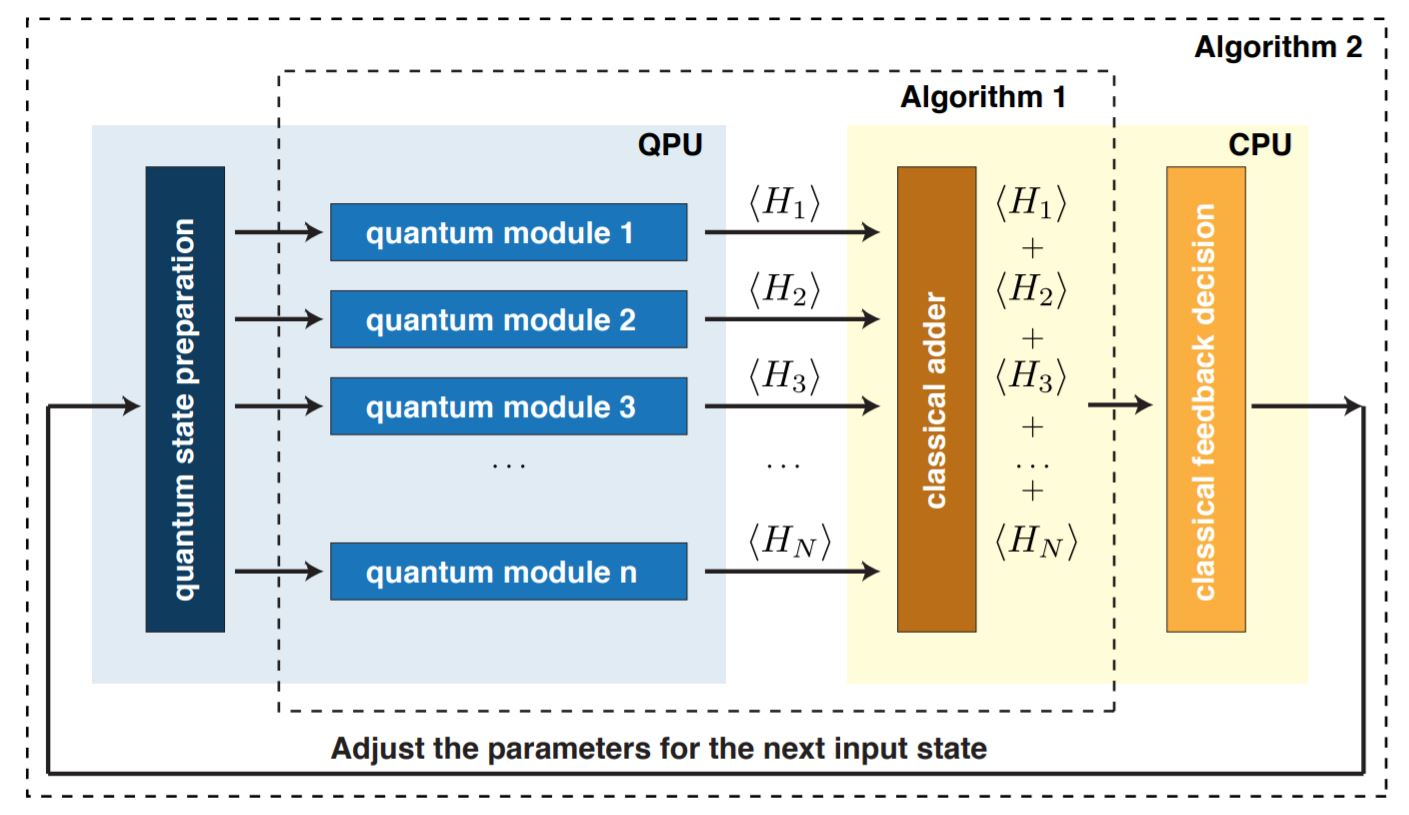
\includegraphics[scale=0.3]{figures/vqe_idea.jpg}
	\caption{Peruzzo et al. (2013)}
	%  Architecture of the quantum-variational eigensolver. Algorithm 1: Quantum states that have been previously prepared, are fed into the quantum modules which compute <Hi>, where Hi is any given term in the sum defining H. The results are passed to the CPU which computes <H>. Algorithm 2: The classical minimization algorithm, run on the CPU,	takes Hi and determines the new state parameters, which are then fed back to the QPU.
\end{figure}
\end{frame}

\section{Rayleigh quotient}
\begin{frame}{Rayleigh quotient}
The eigenvalue problem can be restated as a variational problem on the \textbf{Rayleigh quotient}
\begin{equation}
	|\psi\rangle_{\text{ground}} = {\arg \min} \frac{\exp{\psi |\mathcal{H}|\psi}}{\exp{\psi|\psi}}
	\label{rayleigh}
\end{equation}
Where $|\phi\rangle$ depends on some set of parameters $\{\theta_i\}$

\end{frame}


\section{Classical part}
\begin{frame}{Classical part - optimisation}
	Algorithm 1 is used as a quantum subroutine of Algorithm 2 (better known as VQE). Also check appendix on p. 7 of Peruzzo et al. (2013)
	\\~\\
	Often the choice is Nelder-Mead (from what I encountered), rather than gradient descent because NM is more robust to non-smooth landscapes.
\end{frame}

\section{VQE and QAOA}
\begin{frame}{VQE and QAOA}
In QAOA we construct a parametrised circuit, based on a cost Hamiltonian $\mathcal{H}_C$, encoding the problem, and a mixer Hamiltonian $\mathcal{H}_B$. From these Hamiltonians we construct unitary operators
\begin{equation}
	U(\mathcal{H}_I,\alpha) \coloneq e^{-i\alpha \mathcal{H}_I}
\end{equation}
where $\alpha$ is some angle and $I$ either designates $C$ (cost) or $B$ (mixer).
\end{frame}

\begin{frame}{VQE and QAOA}
Using these definitions, we can lay out the steps of QAOA
\begin{enumerate}
	\item Start with an initial state; the equal superposition over all bitstrings
	\begin{equation}
		|s\rangle = \frac{1}{\sqrt{2^n}}\sum_{b\in \{0,1\}}|b\rangle
	\end{equation}
	\item Evolve with the cost Hamiltonian using $U(\mathcal{H}_C,\gamma_1)$ over angle $\gamma$
	\item Evolve with the mixer Hamiltonian using $U(\mathcal{H}_C,\beta_1)$ over angle $\beta$
	\item Repeat the previous two steps with different angles $\gamma_i$ and $\beta_i$ respectively, do this $p$ times. This results in the state
	\begin{equation}
		|\vec{\gamma},\vec{\beta}\rangle \coloneq \Pi_{i=1}^p U(\mathcal{H}_B,\beta_i) U(\mathcal{H}_C,\gamma_i)
		\label{qaoa-state}
	\end{equation}
\end{enumerate}
\end{frame}

\begin{frame}{VQE and QAOA}
\begin{enumerate}[5]
	\item We are looking for $2p$ angles $\gamma_1, \dots \gamma_p, \beta_1, \dots \beta_p$ in order to optimise the expectation of the cost Hamiltonian $\mathcal{H}_C$
	\begin{equation}
		F_p \coloneq \exp{\vec{\gamma},\vec{\beta}|\mathcal{H}_C|\vec{\gamma},\vec{\beta}}
	\end{equation}
	\textbf{Note} we can determine these angles however we want. Also note that this is in fact very similar to equation \ref{rayleigh}, namely we are trying to find the ground state of a given operator $$\implies \text{we can use VQE!}$$ 
	
\end{enumerate}
\begin{enumerate}[6]
	\item From the state (\ref{qaoa-state}) determined by these optimzal angles we sample bitstrings. The most probable encodes the approximate optimum.\\~\\
	
	
\end{enumerate}
\end{frame}


\section{Some remarks}
\begin{frame}{Some remarks and things to look into}
\begin{itemize}
\item \textbf{Overkill}
Currently, for the small graphs we can encode are more easily solved using brute force.

\item \textbf{Topology}
I am currently using a simulator / QVM. The topology of actual quantum chips is completely ignored. This is especially relevant for higher $p$

\item \textbf{Noise}
I have yet to look at the influence on noise on both VQE and QAOA. Probably there is already quite some literature on that. It is probably possible to simulate the noise as well

\item \textbf{Classical comparison}
It may be interesing to look at the performance compared to the best classical algorithm, namely Goemans-Williamson. 

\item \textbf{Why use QAOA at all when you can use VQE?}
Apparently you can also VQE to solve Max-Cut problems without using QAOA, have a look here: \url{https://www.quanta.guru/docs/optimization/salesman/salesman/ }

\item \textbf{Scaling of p} How will the problem scale with $p$?
\end{itemize}

\end{frame}


\end{document}
